% Created 2020-07-02 jue 16:47
% Intended LaTeX compiler: pdflatex
\documentclass[presentation,aspectratio=169]{beamer}
\usepackage[utf8]{inputenc}
\usepackage[T1]{fontenc}
\usepackage{graphicx}
\usepackage{grffile}
\usepackage{longtable}
\usepackage{wrapfig}
\usepackage{rotating}
\usepackage[normalem]{ulem}
\usepackage{amsmath}
\usepackage{textcomp}
\usepackage{amssymb}
\usepackage{capt-of}
\usepackage{hyperref}
\usepackage{khpreamble}
\usepackage{amssymb}
\usepackage{tcolorbox}
\DeclareMathOperator{\shift}{q}
\DeclareMathOperator{\diff}{p}
\usetheme{default}
\author{Kjartan Halvorsen}
\date{2020-07-02}
\title{Control Computarizado - La transformada z}
\hypersetup{
 pdfauthor={Kjartan Halvorsen},
 pdftitle={Control Computarizado - La transformada z},
 pdfkeywords={},
 pdfsubject={},
 pdfcreator={Emacs 26.3 (Org mode 9.3.6)}, 
 pdflang={English}}
\begin{document}

\maketitle

\section{Intro}
\label{sec:orgaa52c3a}
\begin{frame}[label={sec:org8ede222}]{El mundo según el controlador discreto}
\begin{center}
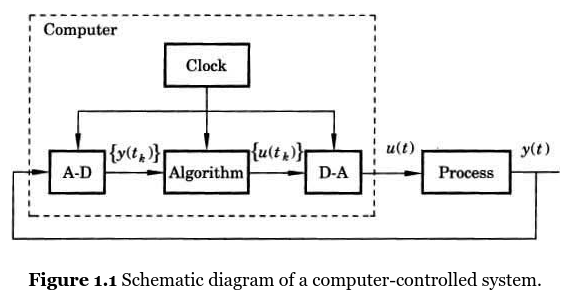
\includegraphics[width=0.6\linewidth]{../../figures/fig1-1-schematic.png}
\end{center}
\end{frame}
\begin{frame}[label={sec:orgf1b2e9c}]{Sistemas muestreados \alert{no} son invariantes en el tiempo continuo}
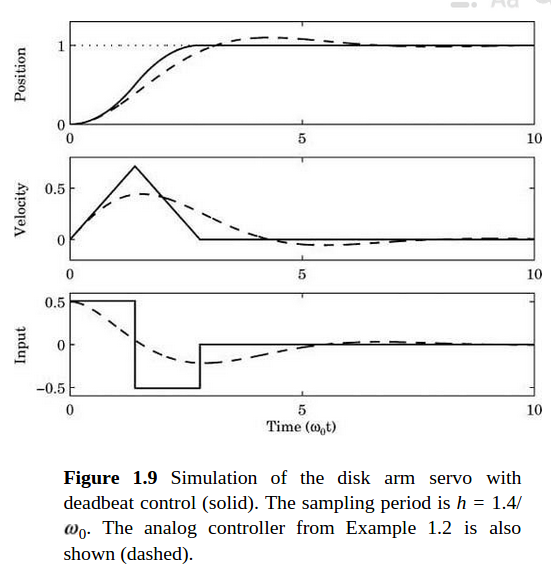
\includegraphics[height=0.6\linewidth]{../../figures/fig1-9.png}
\end{frame}

\begin{frame}[label={sec:orgce825ff}]{Sistemas LTI discretos}
\begin{center}
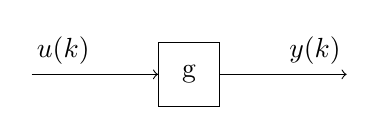
\begin{tikzpicture}[node distance=20mm, anchor=north]
\node[coordinate] (input) {};
\node[rectangle, draw, right of=input, inner sep=3mm] (lti) {g};
\node[coordinate, right of=lti] (output) {};
\draw[->] (input) -- node[near start, above] {$u(k)$}  (lti);
\draw[->] (lti) -- node[near end, above] {$y(k)$} (output);
\end{tikzpicture}
\end{center}
\begin{block}{Caso general (no-causal)}
\[ y(k) = g \ast u = \sum_{n=-\infty}^\infty g(n) u(k-n) \]
\end{block}

\begin{block}{Caso causal}
\[ y(k) = g \ast u = \sum_{n=0}^\infty g(n) u(k-n) \]


\(g(k)\) se llama la \alert{sequencia de ponderación}.
\end{block}
\end{frame}


\begin{frame}[label={sec:orga401d6c}]{Sistemas LTI discretos}
\begin{block}{Respuesta al impulso}
Si la señal de entrada es un impulso unitario

\begin{center}
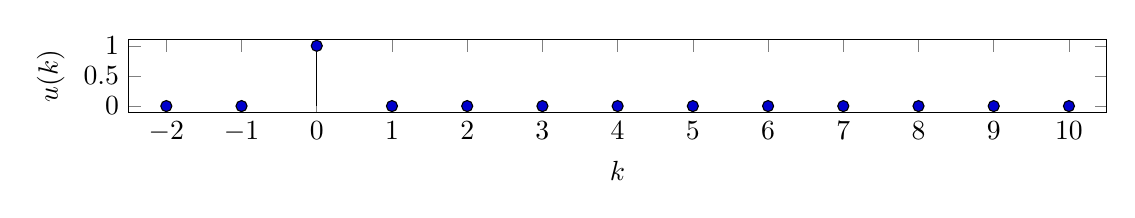
\begin{tikzpicture}
\begin{axis}[
  width=14cm,
  height=2.5cm,
  xlabel={$k$},
  ylabel={$u(k)$},
  xmin=-2.5,
  xmax=10.5,
]

\addplot+[black, ycomb, domain=-2:10, samples=13,variable=k] { (k==0)}; 

\end{axis}
\end{tikzpicture}
\end{center}

\vspace*{-5mm}


\[ y(k) = \sum_{n=0}^\infty g(n) \delta(k-n) = g(k) \]
\end{block}
\end{frame}


\begin{frame}[label={sec:orgf471b95}]{La respuesta de un sistema LSI discreta causal es una suma de valores previod de la señal de entreda}
\[ y(k) = g \ast u = \sum_{n=0}^\infty g(n) u(k-n) \]
La sequencia de ponderación \(g(k)\) es también la respuesta al impulso del sistema. 

\alert{Actividad} Cuál es la respuesta del sistema si la respuesta al impulse es como abajo

\begin{center}
\begin{tikzpicture}
\small
\begin{axis}[
  width=14cm,
  height=3.5cm,
  xlabel={$k$},
  ylabel={$g(k)$},
  xmin=-0.5,
  xmax=10.5,
  ytick = {0, 1},
]

\addplot+[black, ycomb, domain=-2:10, samples=13,variable=k] { (k==4)}; 

\end{axis}
\end{tikzpicture}
\end{center}

\[y(k) = \]
\end{frame}


\begin{frame}[label={sec:orgaf7599e}]{Eigenfunciónes de sistemas LTI discretos}
Si la señal de entrada al sistema es una función exponencial compleja
\[ u(k) = z_1^k, \quad z_1 \in \mathbb{C}  \]
la respuesta será también una función exponencial compleja de la misma forma
\begin{align*}
 y(k) &= \sum_{n=0}^\infty g(n) u(k-n) = \sum_{n=0}^\infty g(n) z_1^{k-n} = \sum_{n=0}^\infty g(n) z_1^{k}z_1^{-n}\\ &=z_1^k \sum_{n=0}^\infty g(n) z_1^{-n} = z_1^k G(z_1).  
 \end{align*}
\end{frame}

\section{La transformada z}
\label{sec:orgff71a59}
\begin{frame}[label={sec:orge7fd2fc}]{La transformada de Laplace}
\begin{block}{Definición (ecuación de análisis)}
\[ F(s) = \laplace{f(t)} = \int_0^\infty f(t) \mathrm{e}^{-st} dt\]
\end{block}
\begin{block}{Transformada inversa (ecuación de síntesis)}
\[ f(t) = \mathcal{L}^{-1}\{F(s)\} = \frac{1}{2\pi i} \int_{\gamma - i\infty}^{\gamma + i\infty} F(s)\mathrm{e}^{st} \, ds \]
\end{block}
\end{frame}

\begin{frame}[label={sec:org4b158ad}]{La transformada z}
\begin{block}{Definición (ecuación de análisis)}
\[ F(z) = \ztrf{f(kh)} = \sum_{k=0}^{\infty} f(kh)z^{-k} \]
\end{block}

\begin{block}{Transformada inversa (ecuación de síntesis)}
\[ f(kh) = \frac{1}{2\pi i} \oint_r F(z) z^{k-1} \, dz \]
\end{block}
\end{frame}

\begin{frame}[label={sec:org6b855f6}]{La transformada de Laplace de una señal muestreada}
\[f_s(t) = f(t)m(t) = f(t) \sum_{k=-\infty}^{\infty} \delta(t-kh) = \sum_{k=-\infty}^{\infty} f(t)\delta(t-kh) = \sum_{k=-\infty}^{\infty} f(kh) \delta(t-kh) \]

\begin{align*}
F_s(s) &= \laplace{f_s(t)} = \int_0^\infty \left(\sum_{k=-\infty}^{\infty} f(kh) \delta(t-kh)\right)\mathrm{e}^{-st}\, dt \\
&= \sum_{k=0}^{\infty} \int_0^\infty  f(kh) \delta(t-kh) \mathrm{e}^{-st}\, dt = \sum_{k=0}^{\infty} f(kh) \mathrm{e}^{-skh}\\
&= \sum_{k=0}^{\infty} f(kh) \left(\mathrm{e}^{-sh}\right)^k
\end{align*}
\end{frame}

\begin{frame}[label={sec:org858df9a}]{La transformada de Laplace de una señal muestreada}
Nota:
\begin{align*}
F_s(s) &=  \sum_{k=0}^{\infty} f(kh) \left(\mathrm{e}^{-sh}\right)^k\quad \text{transformada de Laplace}\\
F(z) &= \sum_{k=0}^{\infty} f(kh) z^{-k} \quad \text{transformada z}
\end{align*}

\begin{tcolorbox}
La transformada z de una señal muestreada corresponde a su transformada de Laplace bajo la relación 
\[ z = \mathrm{e}^{sh}\]
entre el dominio $s$ de la transformada de Laplace y el dominio $z$ de la tranformada z.
\end{tcolorbox}
\end{frame}


\begin{frame}[label={sec:orgd76119b}]{La transformada más importante}
\[f(kh) = \alpha^{kh}, \quad \alpha \in \mathbb{C}\]

\begin{align*}
   F(z) &= \ztrf{f(kh)} = \sum_{k=0}^{\infty} f(kh)z^{-k}
   =  \sum_{k=0}^{\infty} \alpha^{kh}z^{-k} =  \sum_{k=0}^{\infty} \left(\alpha^{h}\right)^kz^{-k}\\
   &=  \sum_{k=0}^{\infty} \left(\frac{\alpha^{h}}{z}\right)^{k}
   =  \frac{1}{1 - \frac{\alpha^h}{z}} = \frac{z}{z-\alpha^{h}}, \quad |\frac{\alpha^h}{z}| < 1
\end{align*}

\begin{tcolorbox}
\[ \alpha^{kh} \quad  \overset{\mathcal{Z}}{\longleftrightarrow} \quad \frac{z}{z-\alpha^h} \]
\end{tcolorbox}
\end{frame}


\begin{frame}[label={sec:org5100db5}]{Otras parejas}
\alert{Actividad (manda por Remind)} Usa la definición de la transformada z
\[ F(z) = \ztrf{f(kh)} = \sum_0^\infty f(kh)z^{-k} \] o el resultado
\[ \alpha^{kh} \quad  \overset{\mathcal{Z}}{\longleftrightarrow} \quad \frac{z}{z-\alpha^h} \]
para calcular las siguientes transformadas de señales derechas (son zero para argumentos negativos)

\begin{center}
\begin{tabular}{ll}
\(f(kh)\) & \(F(z)\)\\
\hline
a) \(f(kh)=\beta\) & \\
b) \(f(kh)=(-1)^k\) & \\
c) \(f(kh) = \mathrm{e}^{i\omega_1 kh}\) & \\
d) \(f(kh) =  \delta(k-3)\) & \\
e) \(f(kh) = \cos(\omega_1 kh)\) & \\
\end{tabular}
\end{center}
\end{frame}

\begin{frame}[label={sec:orgc257b4e}]{Otras parejas - solución}
\[ F(z) = \ztrf{f(kh)} = \sum_0^\infty f(kh)z^{-k} \] o el resultado
\[ \alpha^{kh} \quad  \overset{\mathcal{Z}}{\longleftrightarrow} \quad \frac{z}{z-\alpha^h} \]

\begin{center}
\begin{tabular}{lll}
\(f(kh)\) & \(F(z)\) & Comentario\\
\hline
a) \(f(kh)=\beta\) & \(\beta \frac{z}{z-1}\) & \(f(kh) = \beta (1)^{kh}\)\\
b) \(f(kh)=(-1)^k\) & \(\frac{z}{z+1}\) & \(\alpha^h = -1\)\\
c) \(f(kh) = \mathrm{e}^{i\omega_1 kh}\) & \(\frac{z}{z - \mathrm{e}^{i\omega_1h}}\) & \\
d) \(f(kh) =  \delta(k-3)\) & \(\sum_{k=0}^\infty \delta(k-3)z^{-k} = z^{-3}\) & \\
e) \(f(kh) = \cos(\omega_1 kh)\) & \(\frac{z(z-\cos\omega_1h)}{z^2 - 2\cos(\omega_1h) z + 1}\) & \(\cos\omega_1h = \frac{1}{2}\mathrm{e}^{i\omega_1 h} + \frac{1}{2} \mathrm{e}^{-i\omega_1h}\)\\
\end{tabular}
\end{center}
\end{frame}



\begin{frame}[label={sec:orgac424b4}]{Propiedades básicas de la transformada z}
\begin{center}
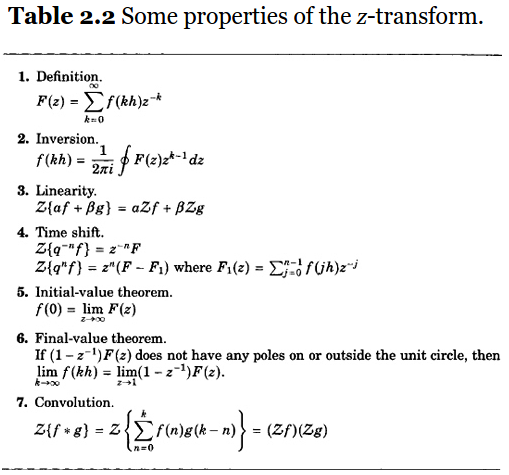
\includegraphics[height=0.8\textheight]{../../figures/table2-2.png}
\end{center}
\end{frame}


\section{Solución de sistemas discretos}
\label{sec:org81d1523}
\begin{frame}[label={sec:orga87c14c}]{Solución de sistemas discretos}
Aplicando la transformada z a la ecuación en diferencias
\[ \left( \shift^2 + a_1\shift + a_2) y_k = \left(b_0\shift^2 + b_1\shift + b_2 \right) u_k\]
da
\begin{equation*}
\begin{split}
z^{2}Y -z^2y(0) &- zy(1) + a_1zY - a_1zy(0) + a_2Y =\\
&     b_0z^2U -b_0z^2u(0) - b_0zu(1) + b_1zU - b_1zu(0) + b_2U
\end{split}
\end{equation*}

\begin{equation*}
\begin{split}
 Y(z) &= \underbrace{ \frac{ \big( y(0)-b_0u(0)\big) z^2 + \big(y(1)+a_1y(0) - b_0u(1) -b_1u(0)\big) z}{z^2 + a_1z + a_2}}_{\text{respuesta transiente}}\\
 & \qquad + \underbrace{\underbrace{\frac{b_0z^2 + b_1z + b_2}{z^2 + a_1z + a_2}}_{\text{función de transferencia}}U(z)}_{\text{respuesta a la señal de entrada}}
\end{split}
\end{equation*}
\end{frame}

\begin{frame}[label={sec:org6792b28}]{Solución de sistemas discretos}
In general, la respuesta de un LTI discreto 

\[ \left( \shift^n + a_1 \shift^{n-1} + \cdots + a_n \right) y(k) = \left( b_0 \shift^m + b_1\shift^{m-1} + \cdots + b_m \right)  u(k) \]

es
\[ Y(z) = \frac{\beta(z)}{A(z)} + \frac{B(z)}{A(z)} U(z) \]

Cuando el sistema está inicialmente relajado: 

\[ Y(z) = \frac{B(z)}{A(z)} U(z)  = G(z) U(z) \]
\end{frame}

\begin{frame}[label={sec:orgd467606}]{Convolución en dominio de tiempo es multiplicación en dominio de z}
\[ \ztrf{g \ast u)} = \ztrf{g(kh)} \ztrf{u(kh)} = \left(\sum_{k=0}^{\infty} g(kh)z^{-k}\right) \left(\sum_{k=0}^{\infty} u(kh)z^{-k}\right)\]


\begin{center}
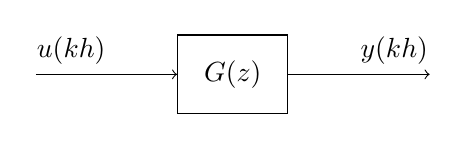
\begin{tikzpicture}[node distance=25mm]
\node[rectangle, draw, minimum height=10mm, minimum width=14mm] (sys) {$G(z)$};
\node[coordinate, left of=sys] (input) {};
\node[coordinate, right of=sys] (output) {};
\draw[->] (input) -- node [near start, above] {$u(kh)$} (sys);
\draw[->] (sys) -- node [near end, above] {$y(kh)$} (output);
\end{tikzpicture}
\end{center}
\[ y(kh) = g(kh) \ast u(kh) \]
\[ \ztrf{y(kh)} = \ztrf{g(kh) \ast u(kh)} \]
\[ Y(z) = G(z) U(z). \]

\begin{tcolorbox}
La transformada z juega el mismo papel para sistemas discretos, como juega la transformada de Laplace para sistemas continuosas!
\end{tcolorbox}
\end{frame}

\begin{frame}[label={sec:orge20bb35}]{Ejemplo: Controlador discreto para el brazo del disco duro}
Usando \(J=1\) y  \(h=1\).
\begin{center}
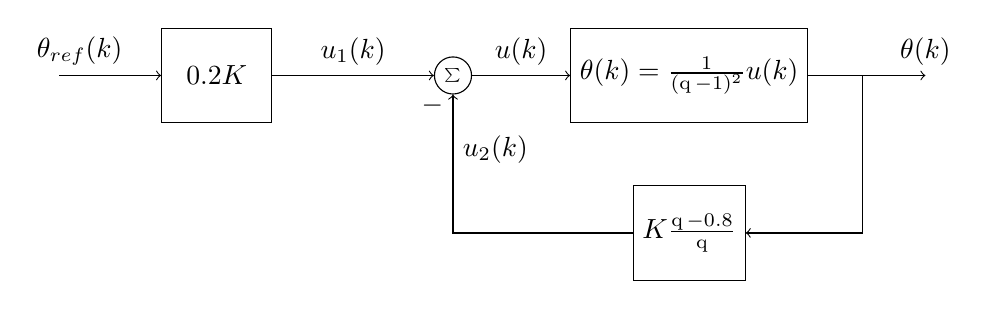
\begin{tikzpicture}
\tikzset{node distance=2cm, 
    block/.style={rectangle, draw, minimum height=12mm, minimum width=14mm},
    sumnode/.style={circle, draw, inner sep=2pt}        
}

  \node[coordinate] (input) {};
  \node[block, right of=input] (TR) {$0.2K$};
  \node[sumnode, right of=TR, node distance=30mm] (sum) {\tiny $\sum$};
  \node[block,right of=sum, node distance=30mm] (plant) {$\theta(k) = \frac{1}{(\shift-1)^2}u(k)$};
  %\node[sumnode, right of=plant, node distance=30mm] (sumdist) {$\sum$};
  %\node[coordinate, above of=sumdist, node distance=15mm] (dist) {};
  %\node[coordinate, right of=sumdist, node distance=15mm] (measure) {};
  \node[coordinate, right of=plant, node distance=30mm] (output) {};
  \node[coordinate, right of=plant, node distance=22mm] (measure) {};
  %\node[sumnode,below of=measure, node distance=25mm] (sumnoise) {$\sum$};
  %\node[coordinate, right of=sumnoise, node distance=15mm] (noise) {};
  \node[block,below of=plant, node distance=20mm] (SR) {$K\frac{\shift - 0.8}{\shift}$};
  \draw[->] (input) -- node[above, pos=0.2] {$\theta_{ref}(k)$} (TR);
  \draw[->] (TR) -- node[above] {$u_1(k)$} (sum);
  \draw[->] (sum) -- node[above] {$u(k)$} (plant);
  \draw[->] (plant) -- node[at end, above] {$\theta(k)$} (output);
  \draw[->] (measure) |- (SR);
  \draw[->] (SR) -| (sum) node[right, pos=0.8] {$u_2(k)$} node[left, pos=0.96] {$-$};
\end{tikzpicture}
\end{center}
Ecuación en diferencias para el sistema de lazo cerrado (usando \(K=0.5\)):
\[ \theta(k+2) - 2\theta(k+1) + \theta(k) = 0.1\theta_{ref}(k) - 0.5\big(\theta(k) -0.8\theta(k-1)\big) \]
\[ \theta(k+3) -2\theta(k+2) + 1.5\theta(k+1) - 0.4\theta(k) = 0.1\theta_{ref}(k+1)\]
\end{frame}

\begin{frame}[label={sec:orga566d09}]{Ejemplo: Controlador discreto para el brazo del disco duro}
\begin{center}
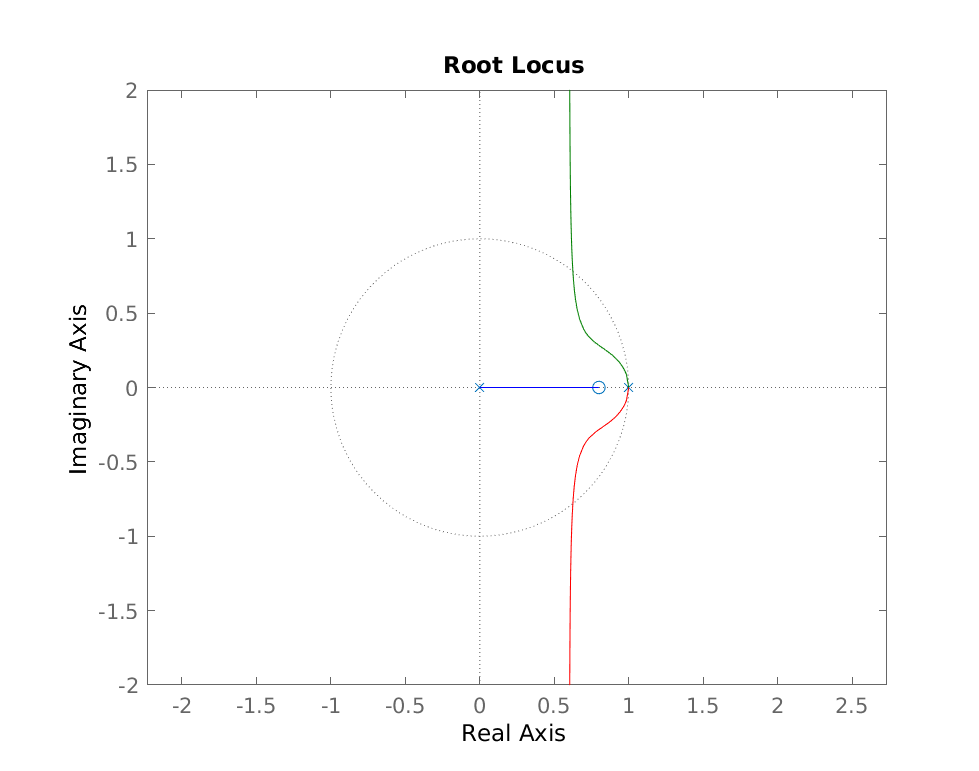
\includegraphics[width=0.7\linewidth]{rlocus-disk-arm.discrete}
\end{center}
\end{frame}

\begin{frame}[label={sec:org4f3e2bb}]{Ejemplo: Controlador discreto para el brazo del disco duro}
Calcula el respuesta a un escalón unitario en \(\theta_{ref}(k)\)! Tenemos
\[ \theta(k+3) -2\theta(k+2) + 1.5\theta(k+1) - 0.4\theta(k) = 0.1\theta_{ref}(k+1)\]
Tomando la transformada z
\[(z^3 - 2z^2 + 1.5z - 0.4) \Theta (z) = 0.1z \Theta_{ref}(z) = 0.1 \frac{z^2}{z-1}\]
\[ \Theta(z) = 0.1 \frac{z^2}{(z-1)(z^3 - 2z^2 + 1.5z - 0.4)} \]
\[ \theta(k) = \mathcal{Z}^{-1}\{\Theta(z)\} = \mathcal{Z}^{-1}\left\{0.1 \frac{z^2}{(z-1)(z^3 - 2z^2 + 1.5z - 0.4)}\right\}\]
\end{frame}
\begin{frame}[label={sec:org3268890}]{Ejemplo: Controlador discreto para el brazo del disco duro}
Solución usando expansión de fracciones parciales:
   \begin{align*}
    \Theta(z) &= 0.1 \frac{z^2}{(z-1)(z^3 - 2z^2 + 1.5z - 0.4)}\\ &= 0.1\frac{z^2}{(z-1)(z-0.62)(z-0.69+0.41i)(z-0.69-0.41i)}\\
    &= 0.1\frac{z^2}{(z-1)(z-0.62)(z^2 -1.38z + 0.64)}\\
    &= \frac{A}{z-1} + \frac{B}{z-0.62} + \frac{Cz + D}{z^2 -1.38z + 0.64}
\end{align*}

\[A = \lim_{z\to 1} (z-1) \Theta(z) = 1.01, \quad etc.\]

\[ \Theta(z) = \frac{1.01}{z-1} - \frac{0.60}{z-0.62} + \frac{0.03-0.41z}{z^2 - 1.38z + 0.64}\]
\end{frame}
\begin{frame}[label={sec:org416d719}]{Ejemplo: Controlador discreto para el brazo del disco duro}
\[ \Theta(z) = \frac{1.01}{z-1} - \frac{0.60}{z-0.62} + \frac{0.03}{z^2 - 1.38z + 0.64} - \frac{0.41z}{z^2 - 1.38z + 0.64}\]
Aplicando la transformada z inversa (ayuda de Wolfram) para cada uno de los terminos
\[
    \theta(k) &= 1.01u_s(k-1) - 0.60(0.62)^{k-1} - 0.05(0.8)^k\Big(\cos(0.53k) + 19.9\sin(0.53 k)\Big)
    \]

\begin{center}
  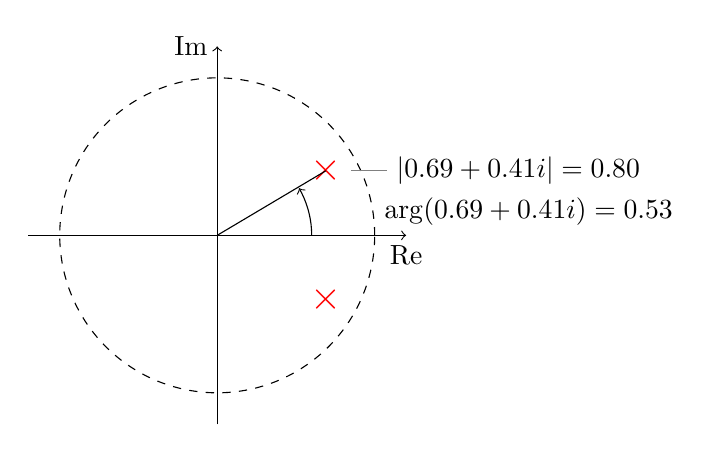
\begin{tikzpicture}[scale=2]
    \draw[->] (-1.2, 0) -- (1.2,0) node[below] {Re};
    \draw[->] (0, -1.2) -- (0,1.2) node[left] {Im};
    \draw[domain=0:360, samples=361, dashed] plot ({cos(\x)}, {sin(\x)});
    \node[red, pin=0:{$|0.69+0.41i|=0.80$}] (pole1) at (0.69, 0.41) { \Large $\times$};
    \node[red] (pole2) at (0.69, -0.41) { \Large $\times$};
    \draw[domain=0:30, samples=10, ->] plot ({0.6*cos(\x)}, {0.6*sin(\x)});
    \node[anchor=west] at (1.0, 0.15) {$\arg (0.69 + 0.41i) = 0.53$};
    \draw[thin] (0,0) to (0.69, 0.41);
    %\node[] at (0.69, -0.2) {$0.69$};
    %\node[] at (0, 0.41) {$0.41 i$};
  \end{tikzpicture}
\end{center}
\end{frame}

\begin{frame}[label={sec:org170387e}]{Ejercicio}
La ecuación en diferencias para el compensador \emph{lead} \(F(s)=K\frac{s+b}{s+a}\) que vímos en la primera clase
\begin{center}
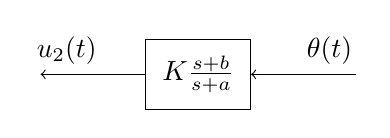
\begin{tikzpicture}
\node[draw, inner sep=6pt] (block) {$K\frac{s+b}{s+a}$};
\draw[->] (block) ++ (2,0) -- node[above, near start] {$\theta(t)$} (block);
\draw[->] (block) -- node[above, near end] {$u_2(t)$}  ++(-2,0);
\end{tikzpicture}
\end{center}
era (con los valores  \(a=8\), \(b=1\), \(h=0.1\), \(K=1\))
\[ u_2(k+1) - 0.2u_2(k) = \theta(k+1) - 0.9\theta(k) \]

\alert{Calcula la respuesta del sistema a una señal escalón unitario.} 
\end{frame}
\end{document}